
\author{Fulya Ozcan}
\documentclass[9pt]{article}
\usepackage{graphicx}
\usepackage{enumitem}% http://ctan.org/pkg/enumitem
\usepackage[margin=1in]{geometry}
\usepackage{setspace}
\usepackage[utf8]{inputenc}
\usepackage{hyperref}
\usepackage{rotating}
\usepackage{amsmath}
\usepackage{algorithm}
\usepackage[noend]{algpseudocode}
\usepackage[english]{babel}
\usepackage[utf8x]{inputenc}
\usepackage{dsfont}
\usepackage{color}
\usepackage[usenames,dvipsnames]{xcolor}

\usepackage{mdframed}
\usepackage{listings}

\definecolor{darkturquoise}{rgb}{0.0, 0.81, 0.82}
\definecolor{coralred}{rgb}{1.0, 0.25, 0.25}
\definecolor{brightturquoise}{rgb}{0.03, 0.91, 0.87}
\definecolor{mygreen}{rgb}{0,0.6,0}
\definecolor{mygray}{rgb}{0.5,0.5,0.5}
\definecolor{mymauve}{rgb}{0.58,0,0.82}


\usepackage{verbdef}% http://ctan.org/pkg/verbdef
\verbdef{\vtext}{verb text}


\lstset{ %
  backgroundcolor=\color{white},   % choose the background color
  basicstyle=\footnotesize,        % size of fonts used for the code
  breaklines=true,                 % automatic line breaking only at whitespace
  captionpos=b,                    % sets the caption-position to bottom
  commentstyle=\color{mygreen},    % comment style
  escapeinside={\%*}{*)},          % if you want to add LaTeX within your code
  keywordstyle=\color{blue},       % keyword style
  stringstyle=\color{mymauve},     % string literal style
  numbers=left, 
  numberstyle=\small, 
  numbersep=8pt, 
  frame = single, 
  language=Pascal, 
  framexleftmargin=15pt
}


\usepackage{tikz}

%\usepackage{factor}

\singlespacing
\begin{document}
   \pagestyle{empty}


\section{Data Description and Feature Reduction}


The data set contains 954 observations (patients) with 1654 possible features.There are 11 main feature sets: Demographics, Comorbidities, T\_Baseline, T\_Concentration, Baseline, Concentration, Max cluster size, Min cluster size, Max cluster T\_Baseline, Min cluster T\_Baseline.


There are two challenges with this data set. The first challenge is that most columns have missing values. Some columns have more than 90\% of their values missing, that is because some patients did not have those measurements. The following figure shows the missing values (black) in the T\_Baseline feature set as an example.

\begin{figure}[ht]
	
	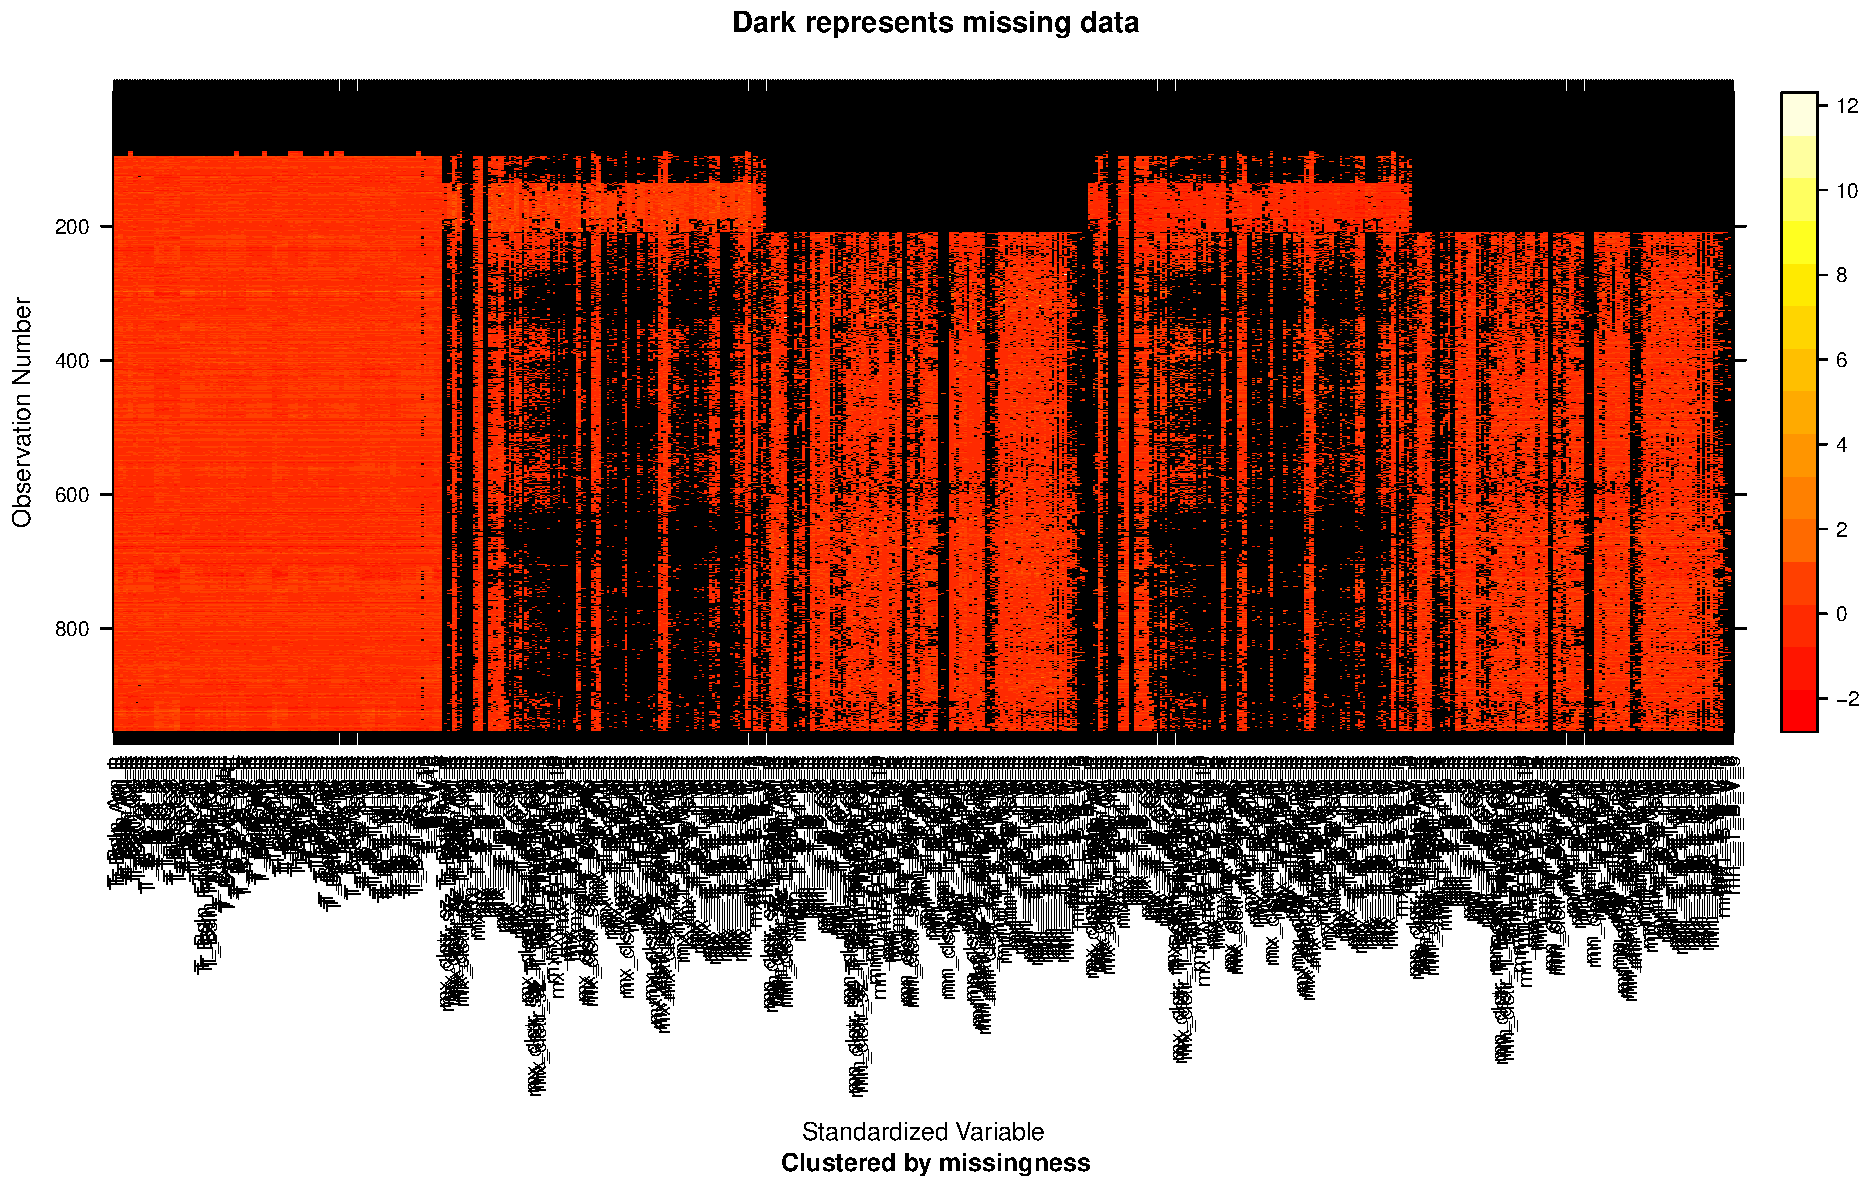
\includegraphics[width=7.3in,height=4in]{missing.pdf}
	\caption{\footnotesize Columns with missing values in T\_Baseline feature set}
\end{figure}

In order to be able to continue our analysis and reduce the noise, we eliminated the missing values in the following way. We first removed the columns that had more than 90\% missing values, since they provide information for only a few patients in the data set. Then, we imputed the remaining missing values using Gelman's \texttt{mi} package in R, which imputes the missing values in an approximate Bayesian framework. This strong imputation technique allowed us to continue our analysis without losing any information. 


The second challenge with this data set was that there were 1654 possible features that we could use, some of which were the different versions of the SPEC readings. We focused our analysis on T\_Baseline feature set from the SPEC data.

Next, to decide which columns (brain regions) in the T\_Baseline feature set are important in terms of their effect on co-diagnoses, we did recursive feature elimination. What this algorithm does is that it finds the important features by repeatedly constructing a model and removing the features that have low importance. We determined 10 important co-diagnoses which for depression, and found which brain regions were affecting them. These co-diagnoses were Anxiety Disorder, Childhood Disorder, Attention Deficit Disruptive Behavior, ADHD, Substance Abuse Disorder, Temporal Dysfunction, Frontal Lobe Dysfunction, Diagnosed Brain Trauma, GAD, PTSD 

As a result of the recursive feature elimination, we identified 10 regions for each co-diagnoses:

\begin{table}[h!]
	\centering
	\begin{small}
	\begin{tabular}{|l|} 
		\hline
\textbf{ Anxiety Disorder }\\\hline
T\_Baseline\_Cerebellum\_Crus2\_R,T\_Baseline\_Parietal\_Sup\_R, T\_Baseline\_Temporal\_Inf\_Post\_L,\\ T\_Baseline\_Vermis\_8, T\_Baseline\_Occipital\_Inf\_R, T\_Baseline\_Occipital\_Inf\_L,    \\ 
T\_Baseline\_Precentral\_R,T\_Baseline\_Postcentral\_R, T\_Baseline\_Cerebellum\_Crus1\_L, T\_Baseline\_Occipital\_Sup\_L \\ \hline   
 \textbf{Childhood Disorder} \\ \hline
  T\_Baseline\_Frontal\_Mid\_Orb\_R\_10, T\_Baseline\_Cerebellum\_7b\_R,
 T\_Baseline\_Cerebellum\_8\_L,   \\ T\_Baseline\_Paracentral\_Lobule\_L,
  T\_Baseline\_Hippocampus\_R,      T\_Baseline\_Pallidum\_L,      \\    
 T\_Baseline\_Putamen\_L,         T\_Baseline\_Frontal\_Inf\_Orb\_R, 
 T\_Baseline\_Temporal\_Inf\_Ant\_R,   T\_Baseline\_Amygdala\_L \\\hline         
\textbf{ Attention Deficit Disruptive Behavior}\\\hline
 T\_Baseline\_Cerebellum\_7b\_R,    T\_Baseline\_Cerebellum\_8\_L,   
 T\_Baseline\_Frontal\_Mid\_Orb\_R\_10, \\ T\_Baseline\_Amygdala\_L, 
 T\_Baseline\_Paracentral\_Lobule\_L, T\_Baseline\_Frontal\_Mid\_Orb\_L\_9 
 T\_Baseline\_Pallidum\_R, \\        T\_Baseline\_Temporal\_Inf\_Post\_R,
T\_Baseline\_Caudate\_L,     T\_Baseline\_Temporal\_Inf\_Ant\_R \\ \hline
 \textbf{ADHD}\\\hline
 [T\_Baseline\_Frontal\_Inf\_Orb\_R,  T\_Baseline\_Frontal\_Mid\_Orb\_R\_10,
T\_Baseline\_Cerebellum\_7b\_R,\\ T\_Baseline\_Hippocampus\_R, 
 T\_Baseline\_Cerebellum\_8\_L,  T\_Baseline\_Temporal\_Mid\_Ant\_R,\\
 T\_Baseline\_Angular\_R,      T\_Baseline\_Hippocampus\_L,    
 T\_Baseline\_Paracentral\_Lobule\_L, T\_Baseline\_Cerebellum\_Crus1\_L \\ \hline
\textbf{ Substance Abuse Disorder}\\ \hline
T\_Baseline\_Heschl\_L,      T\_Baseline\_Temporal\_Sup\_Post\_R, 
 T\_Baseline\_Paracentral\_Lobule\_L,\\ T\_Baseline\_Hippocampus\_L,       
 T\_Baseline\_Calcarine\_L,          T\_Baseline\_SupraMarginal\_R,\\     
T\_Baseline\_Temporal\_Mid\_Post\_R,  T\_Baseline\_Cerebellum\_3\_R,      
T\_Baseline\_Temporal\_Inf\_Ant\_L,   T\_Baseline\_Vermis\_6\\        \hline    
\textbf{ Temporal Dysfunction}\\\hline
 T\_Baseline\_Amygdala\_R,  T\_Baseline\_Vermis\_6,      
 T\_Baseline\_Cingulum\_Mid\_R,\\ T\_Baseline\_Lingual\_L, T\_Baseline\_Insula\_L, T\_Baseline\_Caudate\_L\\ \hline
\textbf{Frontal Lobe Dysfunction}\\\hline
 T\_Baseline\_Cingulum\_Ant\_R,    T\_Baseline\_Cingulum\_Mid\_R ,    T\_Baseline\_Cerebellum\_Crus2\_R,\\
 T\_Baseline\_Rectus\_R, T\_Baseline\_Putamen\_R,         
 T\_Baseline\_Temporal\_Inf\_Ant\_R,\\ T\_Baseline\_Cingulum\_Ant\_L,     T\_Baseline\_Cerebellum\_Crus2\_L,
 T\_Baseline\_Frontal\_Mid\_Orb\_R\\ \hline
\textbf{ Diagnosed Brain Trauma}\\ \hline
 T\_Baseline\_Cerebellum\_8\_R,      
 T\_Baseline\_Temporal\_Mid\_Ant\_L,   T\_Baseline\_Paracentral\_Lobule\_R,\\
 T\_Baseline\_Cingulum\_Ant\_L,       T\_Baseline\_Amygdala\_R ,         
T\_Baseline\_Frontal\_Sup\_Medial\_L,\\ T\_Baseline\_Frontal\_Sup\_Orb\_R,  
 T\_Baseline\_Temporal\_Sup\_Ant\_R,  T\_Baseline\_Amygdala\_L  \\\hline        
\textbf{GAD}\\\hline
T\_Baseline\_Frontal\_Mid\_R,        T\_Baseline\_Temporal\_Inf\_Mid\_L , 
 T\_Baseline\_Occipital\_Inf\_L,      T\_Baseline\_Cerebellum\_Crus2\_L,\\  
T\_Baseline\_Caudate\_R,            T\_Baseline\_Cerebellum\_3\_R,      
T\_Baseline\_Frontal\_Sup\_Medial\_R,\\ T\_Baseline\_Frontal\_Sup\_R,       
T\_Baseline\_Frontal\_Mid\_Orb\_R\_10, T\_Baseline\_Occipital\_Sup\_L\\  \hline   
\textbf{ PTSD}\\ \hline
T\_Baseline\_Cingulum\_Ant\_R,      T\_Baseline\_Frontal\_Inf\_Oper\_L, 
T\_Baseline\_Supp\_Motor\_Area\_L,\\   T\_Baseline\_Cerebellum\_Crus1\_R, 
 T\_Baseline\_Temporal\_Inf\_Mid\_R,  T\_Baseline\_Temporal\_Pole\_Sup\_R,\\
T\_Baseline\_Temporal\_Mid\_Ant\_R , T\_Baseline\_Parietal\_Inf\_R ,    
T\_Baseline\_Supp\_Motor\_Area\_R,   T\_Baseline\_Temporal\_Inf\_Ant\_L\\\hline

 \end{tabular}
\end{small}
	\caption{\footnotesize Important features for co-diagnoses}
\end{table}


After identifying important regions for co-diagnoses, we also identified  significant brain regions that affect the outcome using logistic regression. The 9 significant regions at 5\% level from logistic regression were: Cerebellum\_9\_L, Cingulum\_Post\_L,Fusiform\_L,Fusiform\_R,Pallidum\_L, SupraMarginal\_L,Temporal\_Mid\_Post\_L, Temporal\_Mid\_Post\_R, Temporal\_Pole\_Sup\_L,Vermis\_3.
\end{document}